%\epigraph{Yesterday's rose stands only in name, we hold only empty names.}{--- \textup{Umberto Eco}, \textit{The Name of Rose}}

\subsection{Discovery of Neutrino}
The existence of neutrinos was first put forward by Wolfgang Pauli in the 1930s to solve the contradictions observed in beta decay experiments. It was shown definitively by James Chadwick in 1914 that the electrons emitted in beta decay did not have a discrete set of energies but instead had a continuous spectrum\cite{leite1996weak}. This means that the energy, momentum and angular momentum (spin) were not conserved between the nucleus and electron. To solve this problem, Wolfgang Pauli introduced a charge-neutral, spin-1/2 and nearly massless new particle. The sum of the energies of the new particle, the nucleus and electron is constant, which solved the problem. 

In 1934, Bethe and Peierls suggested direct neutrino detection via a neutrino-induced interaction, called the inverse beta decay (IBD): $\bar{\nu}_e+p\to e^+ + n$. Their calculation showed that the IBD cross section was of the order of $10^{-44}$ cm$^2$. Such a small cross section indicates that the neutrino is difficult to detect\cite{bethe1934neutrino}.

In 1956, Fred Reines and Clyde Cowan made the first discovery of the neutrino (specifically, it was electron antineutrinos $\bar{\nu}_e$) by using a nuclear reactor as an intense neutrino source with neutrino fluxes on the order of $10^{12}-10^{13}$ neutrinos/second/cm$^2$. The active volume of their detector was two tanks filled with water in which cadmium chloride (CdCl$_2$) was dissolved. The water tanks were surrounded by liquid scintillator layers coupled with photomultiplier tubes (PMT) to detect emitted photons. The incoming antineutrinos interacted with the water via IBD. The produced positrons quickly annihilated with $e^-$ and gave $\gamma$ signals while the produced neutrons went through the neutron capture process: $n+^{108}$Cd$\to^{109}$Cd$^*\to^{109}$Cd$+\gamma$ and gave delayed $\gamma$ signals. A coincidence of these two characteristic signals provided a distinctive signature for the neutrino reaction. They measured the cross-section as $6.3\times10^{-44}$ cm$^2$, which was consistent with Bethe's calculation\cite{reines1960detection}.

\subsection{Solar Neutrino}
In the 1930s, Hans Bethe et al. explained the origin of the Sun's energy as a series of nuclear reactions\cite{bethe1939energy}.

Based on the available physics and experimental data, the Standard Solar Model (SSM) is a modern accepted theory for the evolution of the Sun. The energy in the Sun is mainly produced by two classes of reactions: the proton-proton (pp) chain and the Carbon-Nitrogen-Oxygen (CNO) cycle. The result of the two reactions is: $4p+2e^-\to^{4}$He$+2\nu_e+Q$, where the released energy, $Q$ is 26.73 MeV. The $\nu_e$ produced in the Sun (the solar neutrinos) can be detected on the Earth\cite{giunti2007fundamentals}.

Due to the branching ratios and unterminated chains in the pp chain and CNO cycle, the solar neutrinos come from different reactions, as shown in Table~\ref{solarnu}. The solar neutrinos detected on the Earth are named after the specific fusion process\cite{haxton2013solar}. They have different fluxes and energies, as shown in Figure~\ref{bp05plot}\cite{bahcall2005new}.

\begin{table}[htp]
	\caption[]{\label{solarnu} Solar neutrinos from reactions in pp chain (a) and CNO cycle (b).}	
	\subfigure[pp chain]{
		\begin{tabular*}{62mm}{cc}
			\toprule 
			solar $\nu_e$  & reaction  \\
			\midrule
			pp & $p+p\to ^2$H $+e^++\nu_e$ \\
			pep & $p+e^-+p\to^2$H $+~\nu_e$ \\
			hep &  $^3$He $+~p\to^4$He $+~e^++\nu_e$ \\ 
			$^7$Be &  $^7$Be $+~e^-\to^7$Li $+~\nu_e$\\
			$^8$B & $^8$B$\to^8$Be$^*+e^++\nu_e$\\
			\bottomrule	
		\end{tabular*}
	}
	\subfigure[CNO cycle]{
		\begin{tabular*}{60mm}{cc}
			\toprule 
			solar $\nu_e$   & reaction \\
			\midrule
			CNO &$^{13}$N$\to^{13}$C$+e^++\nu_e$\\	
			& $^{15}$O$\to^{15}$N$+e^++\nu_e$ \\
			& $^{17}$F$\to^{17}$O$+e^++\nu_e$ \\
			\bottomrule	
		\end{tabular*}
	}
\end{table}

\begin{figure}[htbp]
	\centering	
	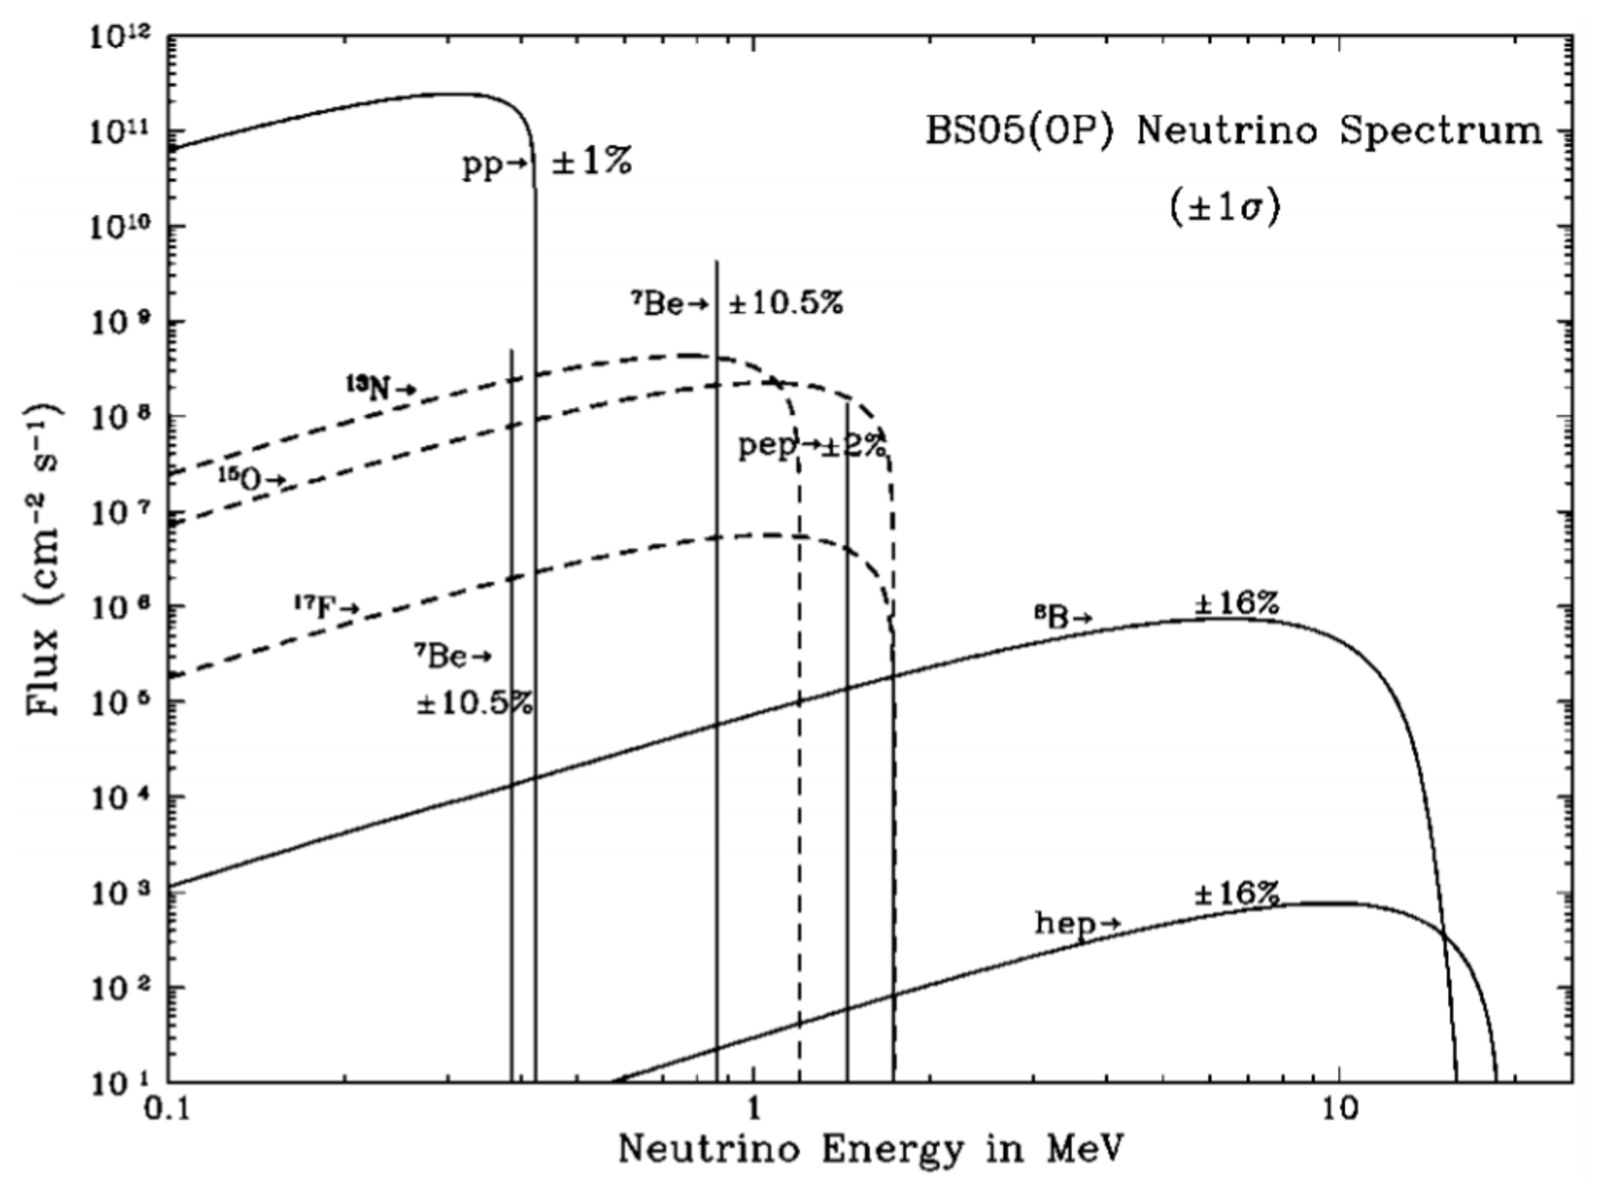
\includegraphics[width=10cm]{BP05.pdf}
	\caption{ Solar neutrino energy spectrum ($E_\nu$ vs. flux) for the solar model BS05(OP)\cite{BP05}.}
	\label{bp05plot}
\end{figure}

\subsection{Early Solar Neutrino Experiments}
In 1964, John Bahcall and Raymond Davis proposed the first experiment to detect solar neutrinos\cite{bahcall1,raymond}. Raymond Davis designed an experiment that used a 380 m$^3$ tank filled with Perchloroethylene (C$_2$Cl$_4$), a dry-cleaning fluid rich in chlorine. Solar neutrinos were expected to change $^{37}$C1 to $^{37}$Ar via the endothermic reaction $\nu_e+^{37}$Cl$\to^{37}$Ar$+e^-$ and the produced $^{37}$Ar were extracted and counted. The neutrino energy threshold ($E_{thresh}$) of the experiment was 0.814 MeV, which allowed a measurement mostly of the $^8$B neutrino flux but also including some lower energy neutrinos\cite{raymond}. Their first results, announced in 1968, showed that only about one-third of the predicted radioactive argon atoms were measured. This raised a problem of missing solar neutrinos.

\subsection{Atmospheric Neutrino}
Cosmic rays from outer space continuously interact with nuclei in the atmosphere and produce secondary particles. Atmospheric neutrinos come from decay products of the hadrons in the secondaries. The dominant processes of atmospheric $\nu_e$ and $\nu_\mu$ production is $\pi^+\to\mu^+ + \nu_\mu$ followed by $\mu^+ \to e^+ + \bar{\nu}_\mu + \nu_e$. In the 1980s, the Kamiokande experiment in Japan measured atmospheric neutrinos by utilizing a 3-kiloton water-Cherenkov detector. The incoming neutrinos, $\nu_e$ ($\nu_\mu$) interacted with the water via charged current interactions and electrons (muons) were produced. The electrically charged leptons traversed the water at a speed higher than the speed of light in water and thus emit Cherenkov light, which was recorded by the detector as ring patterns (called Cherenkov rings). The produced electrons caused electro-magnetic showers during their propagation in the water while the produced muons propagated almost in straight lines without producing electro-magnetic showers. Then the $\nu_\mu$ (the $\mu$-like events) were separated from the $\nu_e$ (the $e$-like events) by the fact that the $\mu$-like events created sharper Cherenkov rings than the $e$-like events. Kamiokande measured the ratio of fluxes $\Phi(\nu_\mu+\bar{\nu}_\mu)/\Phi(\nu_e+\bar{\nu}_e)$. The fluxes of atmospheric neutrinos are well understood and the ratio $\nu_\mu/\nu_e$ is expected to be $\sim$2 at low energies $\leq$1~GeV. In 1988, they found a deficit of measured $\mu$-like events compared to the prediction. This was later confirmed by IMB in 1992\cite{becker1992electron} and Soudan-2 in 1997\cite{allison1997measurement} and called ``atmospheric neutrino anomaly''\cite{kajita2012atmospheric}.

\section{Neutrino Oscillation and Flavor Transformation}
Neutrino oscillation is a quantum mechanical interference phenomenon\cite{akhmedov2019quantum}. It was first discovered in 1998, based on the analysis of atmospheric neutrino fluxes measured by the Super-Kamiokande (SuperK) experiment to solve the ``atmospheric neutrino anomaly'' mentioned in the last section\cite{fukuda1998evidence}. It is the first direct evidence showing that neutrinos have finite masses and the Standard Model is incomplete.

Based on current knowledge, neutrinos only interact via the weak force and
gravity. A neutrino $\nu_\alpha$ is generated with a definite flavor from weak interaction and is related to a charged lepton with a given flavor: the electron ($e$), the muon ($\mu$) or the tauon ($\tau$) and thus $\alpha=e,\mu,\tau$.

 flavor eigenstates.   

\subsection{Vacuum Oscillation}

\[
|\nu_\alpha>=\sum_{i=1}^n U^*_{\alpha i}|\nu_i>
\]

For three-flavor neutrino mixing, we have\cite{pdg2018}:
\begin{equation}\label{eq:mixingmatrix}
|\nu_f> = \sum_{k=1}^3U^*_{fk}|\nu_k>, 
\end{equation}
where $f=e,\mu,\tau$ and $k=1,2,3$. The unitary PMNS matrix, $U_{PMNS}$, can be parametrized as: 

$U_{PMNS} = $
\begin{equation}
\begin{bmatrix}
1 &0 &0\\
0 &\cos\theta_{23} &\sin\theta_{23}\\
0 &-\sin\theta_{23} &\cos\theta_{23}\\ 
\end{bmatrix}
\begin{bmatrix}
\cos\theta_{13} &0 &e^{-i\delta_{CP}}\sin\theta_{13}\\
0 &1 &0\\
e^{-i\delta_{CP}}\sin\theta_{13} &0 &\cos\theta_{13}\\ 
\end{bmatrix}
\begin{bmatrix}
\cos\theta_{12} &\sin\theta_{12} &0\\
-\sin\theta_{12} &\cos\theta_{12} &0\\
0 &0 &1\\ 
\end{bmatrix}.
\end{equation}


\[
P_{\alpha\beta}=\delta_{\alpha\beta}-4\sum_{i<j}^n Re[U_{\alpha i}U^*_{\beta i}U^*_{\alpha j}U_{\beta j}]\sin^2
\]

In the PMNS matrix, we have four parameters: the three mixing angles $\theta_{12}$, $\theta_{13}$, $\theta_{23}$ and the charge-parity (CP) violation parameter of lepton sector, $\delta_{CP}$. The unknown value of $\delta_{CP}$ is related to leptogenesis, the hypothetical physical process that produced an asymmetry between leptons and antileptons in the very early universe\cite{wiki_cp}. 

In addition, there are two squared-mass differences, $\Delta m^2_{21}=m_2^2-m_1^2$ and $\Delta m^2_{32}=|m_3^2-m_2^2|$. The sign of $\Delta m^2_{32}$ is unknown and it indicates a mass hierarchy problem of whether neutrino mass is normal hierarchy (NH, $m_3>m_2>m_1$) or inverted hierarchy (IH, $m_3<m_1<m_2$)\cite{pdg2018}. 

Currently, these six parameters have been measured by neutrino oscillation experiments. These experiments can be classified by the neutrino sources they use. They are the solar, the reactor, the atmospheric, the accelerator and the astronomical and cosmological neutrino experiments. Table~\ref{nu_exp} lists the energy scale of the neutrino source as well as the example experiments.

\begin{table}[ht]
	\caption{\label{nu_exp} Oscillation neutrino experiments.}	
	{\centering
		\begin{tabular*}{135mm}{c@{\extracolsep{\fill}}cccc}
			\toprule 
			type & source & $E_\nu$ & example\\
			\midrule
			solar& the Sun & MeV scale & SNO \\
			reactor& reactor & MeV scale & DayaBay \\
			atmospheric& cosmic-ray& GeV scale & SuperK\\
			accelerator&  $\nu$ beam from accelerator & GeV scale & T2K\\	
			astronomical& astronomical objects & GeV-EeV scale & IceCube\\	
			\bottomrule	
		\end{tabular*}
	}
\end{table}


For the $\Delta m^2_{21}$ and $\theta_{12}$, the combined analysis of the measurements from the reactor experiment KamLAND and SNO gave $\Delta m^2_{21} = 7.59^{+0.21}_{-0.21}\times 10^{-5}eV^2$ and $\tan^2{\theta}_{21}=0.47^{+0.06}_{-0.05}$\cite{kamland_measure}.

The accelerator neutrino experiments as well as the atmospheric neutrino experiments have measured $\Delta m^2_{32}$ and $\theta_{23}$. The most recent results from SuperK show that in NH, $\sin^2\theta_{23}=0.588^{+0.031}_{-0.064}$ and $\Delta m^2_{32} = 2.5^{+0.13}_{-0.20}\times 10^{-3} eV^2$\cite{superk_new}. 

In 2012, the reactor neutrino experiment Daya Bay reported the discovery of non-zero $\theta_{13}$ with a significance of 5.2$\sigma$. In 2016, Daya Bay reported that $\sin^2 2\theta_{13} = 0.0841\pm0.0027(stat.)\pm0.0019(syst.)$. This high-precision result makes $\sin^2 2\theta_{13}$ the best measured mixing angle\cite{dayabayresults,reactorNu}.

$\delta_{CP}$ is examined by the experiments which measure the difference between neutrino and antineutrino oscillation probabilities $P(\bar{\nu}_\alpha\to\bar{\nu}_\beta)$ and $P(\nu_\alpha\to\nu_\beta)$\cite{xing}. In 2017, the Tokai-to-Kamioka (T2K) experiment in Japan rejected the hypothesis that neutrinos and antineutrinos oscillate with the same probability at 95\% confidence (2$\sigma$) level. This indicates a hint of CP symmetry broken by neutrinos\cite{abe2017measurement}. In 2019, T2K  claimed confidence intervals for $\delta_{CP}$ with three standard deviations ($3\sigma$): [-3.41,-0.03] for NH and [-2.54,-0.32] for IH. This result indicates that the CP violation exists in leptons\cite{abe2019constraint}.


The oscillation probability in matter can be written in a concise and exact form as \cite{kimura2002exact}:
\[
P(\nu_e\to\nu_\mu) = A\cos\delta+B\sin\delta+C
\]



will also provide the information for the CP- and T-violation
by investigating the quantities of:
\[
A_{CP} = \frac{P(\nu_\alpha\to\nu_\beta)-P(\bar{\nu}_\alpha\to\bar{\nu}_\beta)}{P(\nu_\alpha\to\nu_\beta)+P(\bar{\nu}_\alpha\to\bar{\nu}_\beta)}
\]

\[
A_T = \frac{P(\nu_\alpha\to\nu_\beta)-P(\bar{\nu}_\beta\to\bar{\nu}_\alpha)}{P(\nu_\alpha\to\nu_\beta)+P(\bar{\nu}_\beta\to\bar{\nu}_\alpha)}
\]





\subsection{Matter Effect}

The matter effect is caused by neutrinos interacting with ambient electrons and nucleons in matter such as the Sun or the Earth. $\nu_e$ interacts with electrons via both charged weak current (exchanging $W$ boson) and neutral weak current ($Z$ boson) while $\nu_\mu$ and $\nu_\tau$ interact only by the neutral current. The $\nu_e$ energy has an addition term, $V_{CC} =\sqrt2G_Fn_e$, where $n_e$ is the number density of the electrons in matter and $G_F$ is the Fermi coupling constant for the weak interaction. This affects the oscillation probabilities for neutrinos propagating in matter compared to vacuum, which is called the Mikheyev-Smirnov-Wolfenstein (MSW) mechanism\cite{smirnov2016solar,smirnov2005msw}.

In vacuum two-flavor mixing, the Schr\"{o}dinger equation can be written (in natural units)\cite{xing2011neutrinos}:
\begin{equation}\label{eq:2flavor_simple}
	i\frac{d}{dt}\begin{bmatrix}
		\nu_e\\
		\nu_\mu\\
	\end{bmatrix}
	=
	H^f_0
	\begin{bmatrix}
		\nu_e\\
		\nu_\mu\\
	\end{bmatrix},
\end{equation}
where 

\begin{equation} \label{eq:H0f}
\begin{aligned}
 H^f_0 = \frac{1}{2E}\begin{bmatrix}m^2_1\cos^2\theta+m^2_2\sin^2\theta & (m^2_2-m^2_1)\sin\theta\cos\theta \\ (m^2_2-m^2_1)\sin\theta\cos\theta & m^2_1\sin2\theta+m^2_2\cos^2\theta\end{bmatrix} =
\\
\frac{\Delta m_{21}^2}{4E}\begin{bmatrix}
	-\cos 2\theta & \sin 2\theta\\
	\sin 2\theta & \cos 2\theta\\
\end{bmatrix}+\frac{(m_1^2+m_2^2)}{4E}\begin{bmatrix}
	1 & 0\\
	0 &1\\
\end{bmatrix},
\end{aligned}
\end{equation}
and $\Delta m^2_{21}=(m^2_2 - m^2_1)$.

To simplify the calculation, we can drop the second unitary term of $H^f_0$ that is irrelevant to the neutrino flavor transformation. Including the matter effect, we obtain:
\begin{equation}\label{eq:Hm}
	H_m = \begin{bmatrix}
		-\frac{\Delta m_{21}^2}{4E}\cos 2\theta+\sqrt 2G_Fn_e & \frac{\Delta m_{21}^2}{4E}\sin 2\theta\\
		\frac{\Delta m_{21}^2}{4E}\sin 2\theta &\frac{\Delta m_{21}^2}{4E}\cos 2\theta\\
	\end{bmatrix}
\end{equation}

We define a mixing angle in matter, $\theta_m$ as:
\begin{equation}\label{eq:thetaM}
	\tan 2\theta_m = \frac{\Delta m^2\sin2\theta}{\Delta m^2\cos2\theta-2\sqrt 2E G_Fn_e},
\end{equation}
and define an effective squared-mass difference in matter $\Delta m^2_m$ as:
\begin{equation}
	\Delta m^2_m = \sqrt{(\Delta m^2\cos2\theta - 2\sqrt 2EG_Fn_e)^2+(\Delta m^2\sin2\theta)^2}.
\end{equation}

In analogy with mixing in vacuum, we can write the mixing equation relating the energy eigenstates in matter ($\nu_{1m},\nu_{2m}$) to the flavor eigenstates with a diagonalized Hamiltonian:
\begin{equation}\label{eq:matter_mixing}
	\begin{bmatrix}
		\nu_e\\
		\nu_\mu\\
	\end{bmatrix}
	= \begin{bmatrix}
		\cos\theta_m & \sin\theta_m\\
		-\sin\theta_m & \cos\theta_m \\
	\end{bmatrix}
	\begin{bmatrix}
		\nu_{1m}\\
		\nu_{2m}\\
	\end{bmatrix}.
\end{equation}

The probability of flavor transformation in matter is:
\begin{equation}
	P_{\nu_e\to\nu_{\mu}}=\sin^2(2\theta_m)\sin^2\Big(\frac{\Delta m_m^2L}{4E}\Big).
\end{equation}

The denominator in equation (\ref{eq:thetaM}) implies a resonance condition:
\begin{equation}\label{eq:reson_condition}
	V(n_e)=\sqrt 2G_Fn_e=\frac{\Delta m^2\cos2\theta}{2E}.
\end{equation}

From this condition, for a given $E$, there is a resonance density $n^{reson}_e$ while for a given $n_e$, there is a resonance energy $E^{reson}$. When the resonance condition is satisfied, $\theta_m = \frac{\pi}{4}$ and two flavor neutrinos are maximally mixed, even if the vacuum mixing angle $\theta$ is small. This is called matter enhanced neutrino oscillation\cite{smirnov2016solar,fukugita2013physics}.

\subsection{Reactor-solar Experiments}

KamLand

Daya Bay

The Jiangmen Underground Neutrino Observatory (JUNO) is a reactor neutrino experiment located at Kaiping, Jiangmen in Southern China. a large liquid scintillator detector 
large active mass of 20 kton

the energy resolution (3\% at 1 MeV) 
\cite{giaz2018status}

\subsection{Atmosphere-accelerator Experiments}



\subsection{Astrophysics Experiments}
Neutrino telescopes
Ice cube
Baikal 





\section{Majorana Neutrino}

Dirac equation $(i\gamma^\mu\partial_\mu-m)\psi=0$,
get coupled equations


The interpretation of the $0\nu\beta\beta$ process is considered as exchanging light Majorana neutrinos. In this case the effective Majorana mass $<m_{ee}>=\sum_{i=1}^{3} |U_{ei}|^2m_i~(i=1,2,3)$, where $U_{ei}$ are the elements of the neutrino mixing matrix for the flavor state $\nu_e$, and $m_i$ are the mass eigenvalues of the mass eigenstates (from (\ref{eq:mixingmatrix})). The observable quantity is the half-life:
\[
(T^{0\nu\beta\beta}_{1/2})^{-1} = G_{PS}(Q,Z)|M_{Nuclear}|^2<m_{ee}>^2, 
\]



Majorana found a representation of the $\gamma$-matrices as follow:
\[
\gamma_M^0 = \begin{pmatrix} 
0 & \sigma^2 \\
\sigma^2 & 0
\end{pmatrix},
\gamma_M^1 = \begin{pmatrix} 
\sigma^3 & 0 \\
0 & \sigma^3
\end{pmatrix},
\gamma_M^2 = \begin{pmatrix} 
-\sigma^2 & 0 \\
0 & \sigma^2
\end{pmatrix},
\gamma_M^3 = -i\begin{pmatrix} 
\sigma^1 & 0 \\
0 & \sigma^1
\end{pmatrix}
\]


These matrices themselves are pure imaginary. 


For heavy radioactive isotopes with nuclei of even neutron number ($N$) and even proton number ($Z$) (called even-even nucleus), beta decay will lead to an odd-odd nucleus which is less stable. For some such isotopes the beta decay is energetically forbidden. In 1935, Maria Goeppert-Mayer pointed out that they can still decay through a double beta decay process: $(Z,A) \to (Z+2,A)+2e^{-}+2\bar{\nu_e}+Q_{\beta\beta}$, where the $Q_{\beta\beta}$ is the released energy. This is called ordinary double beta decay or $2\nu\beta\beta$, which is allowed by the Standard Model and with a typical half-life $T_{1/2}>10^{19}$ years\cite{martin}.

If neutrinos are Majorana particles, a process called neutrinoless double beta decay ($0\nu\beta\beta$) will also be expected. The Feynman diagrams of $2\nu\beta\beta$ and $0\nu\beta\beta$ are illustrated in Fig.~\ref{feynman1}.

\begin{figure}[htbp]
	\centering	
	\begin{minipage}[t]{0.45\textwidth}
		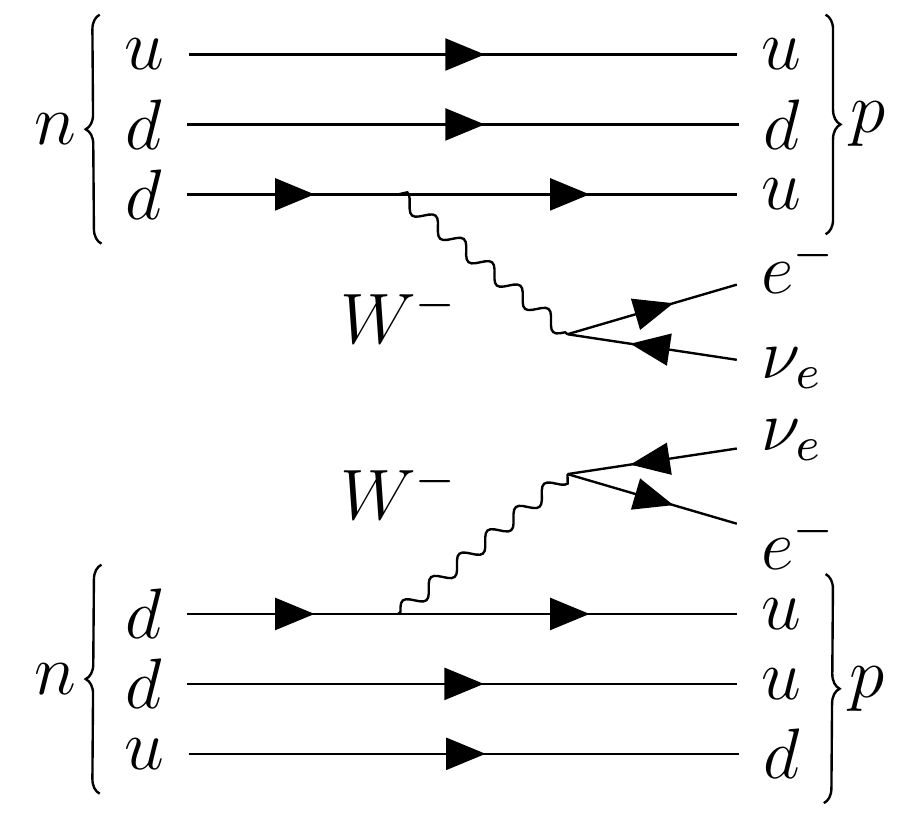
\includegraphics[width=5cm]{doubleBeta2nu_feynman.png}
	\end{minipage}
	\begin{minipage}[t]{0.45\textwidth}
		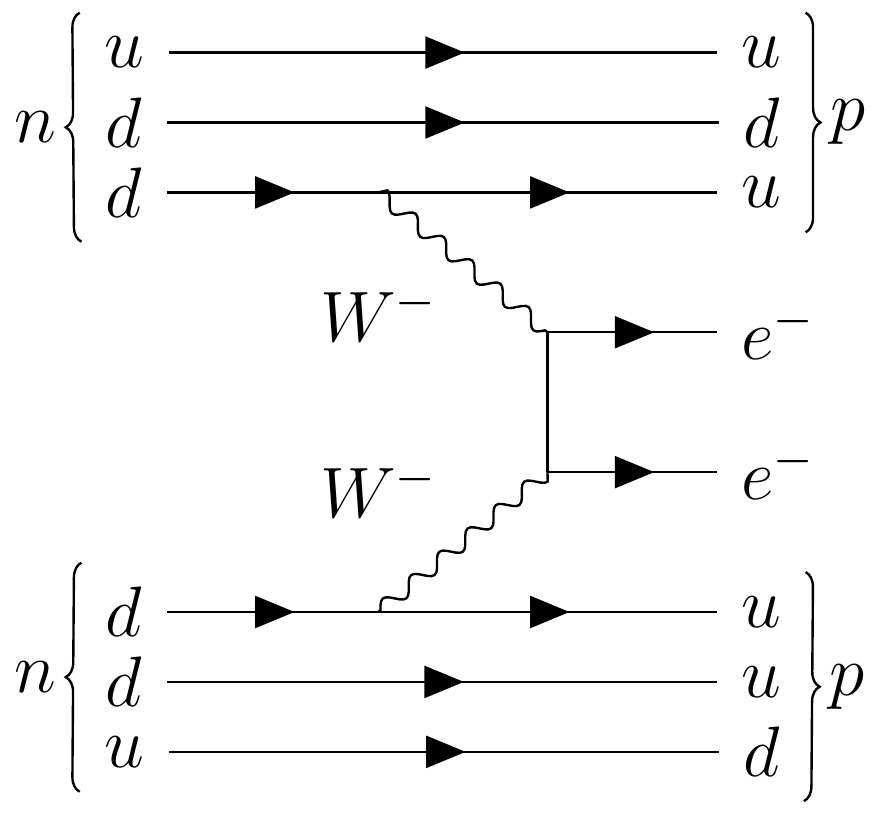
\includegraphics[width=5cm]{doubleBeta_feynman.png}
	\end{minipage}
	\caption{ Feynman diagrams for $2\nu\beta\beta$ (left) and $0\nu\beta\beta$ (right).}
	\label{feynman1}
\end{figure}

The interpretation of the $0\nu\beta\beta$ process is considered as exchanging light Majorana neutrinos. In this case the effective Majorana mass $<m_{ee}>=\sum_{i=1}^{3} |U_{ei}|^2m_i~(i=1,2,3)$, $U_{ei}$ are the elements of the neutrino mixing matrix for the flavor state $\nu_e$, and $m_i$ are the mass eigenvalues of the mass eigenstates (from (\ref{eq:mixingmatrix})). The observable quantity is the half-life:
\[
(T^{0\nu\beta\beta}_{1/2})^{-1} = G_{PS}(Q,Z)|M_{Nuclear}|^2<m_{ee}>^2, 
\]
where $G_{PS}$ is the phase space factor and $|M_{Nuclear}|$ is the nuclear matrix element for the physics process describing the $0\nu\beta\beta$ decay process\cite{zuber2011neutrino}.

Similar to beta decay, the $2\nu\beta\beta$ process will cause a continuous spectrum in the detector while the $0\nu\beta\beta$ process only has two electrons in the final state, which sum up to give a distinct energy peak. By measuring this exact energy, a detector with high energy resolution is able to search for the $0\nu\beta\beta$ signal from the $0\nu\beta\beta$ decay radioactive isotopes. Diverse technologies have been developed during the past decades. The following section lists some of the mainstream experiments.

\begin{equation}\label{eq:majoranaField}
\Psi_R=\begin{bmatrix}
\psi_R\\
\psi_R^C\\
\end{bmatrix},
\Psi_L=\begin{bmatrix}
\psi_L\\
\psi_L^C\\
\end{bmatrix},
M=\begin{bmatrix}
m_L^M &  m^D\\
m^D &  m_R^M\\
\end{bmatrix},
\end{equation}
%
The mass eigenstates:
\[
m_{\pm} = \frac{1}{2}[~(m_L^M+m_R^M)\pm\sqrt{(m_L^M-m_R^M)^2+4(m^D)^2}~]\label{eq:majorana_massEigen},
\]
from (\ref{eq:majorana_massEigen}), there are 4 cases for discussion:\\
(1) If $m_L^M=m_R^M=0$, $m_{1,2}=m^D$, neutrinos are pure Dirac particles.\\
(2) If $m^D\gg m^M_{L,R}$, $\frac{m^D}{m_{L,R}^M}\to 0$, $m_{1,2}=\frac{1}{2}m^D[~\frac{(m_L^M+m_R^M)}{m^D}+\sqrt{(\frac{m^M_L-m^M_R}{m^D})^2+4}~]\approx m^D$, neutrinos are Pseudo-Dirac-Neutrinos.
\\
(3) If $m^D=0$, $m_1=m^M_L, m_2=m^M_R$, neutrinos are pure Majorana particles.\\
(4) In the case of the seesaw mechanism, where $m_R^M\gg m^D, m_L^M=0$,
and for $(\frac{m^D}{m_R^M})^2\to 0$, use $(1+x)^\alpha\sim 1+\alpha x ~~(~if~x\to 0~)$, we get:
\[
m_1=m_-=\frac{\frac{1}{2}[(m^M_R)^2-(m^M_R)^2-4(m^D)^2]}{m_R^M(1+\sqrt{1+4(\frac{m^D}{m^M_R})^2})}\approx -\frac{(m^D)^2}{m^M_R},
\]

\[
m_2=m_+=\frac{1}{2}[m^M_R+m^M_R(1+\frac{1}{2}(\frac{2m^D}{m^M_R})^2)]=m^M_R[1+(\frac{m^D}{m^M_R})^2]\approx m^M_R.
\]


For $\mathcal{O}(1TeV)$, the $\nu$ mass is $0.1~eV$












\subsection{Status of Double Beta Decay Experiments}

There are 35 isotopes can undergo the double beta decay process, but only a few of them are suitable for the application in direct $0\nu\beta\beta$ search experiments\cite{giunti2007fundamentals}. From the experimental view, the candidate isotopes are expected to have relatively high natural abundances, high Q-values, be deployed in a large amount with low costs, and are not toxic to the environment as well. However, in realistic situation there is no isotope fulfills all these properties and the current experiments making trade-offs\cite{dolinski2019neutrinoless}.

The experiments searching for direct signals of $0\nu\beta\beta$ mainly measure the physics properties of the two emitted electrons, such as their energies, momentum and tracks. 

inhomogeneous experiments use external $\beta\beta$ source
while homogeneous experiments use $\beta\beta$ source as the detection medium, which are mainly referred as calorimeter experiments\cite{cremonesi2014challenges,shimizu2019double}.




$^{136}$Xe, $^{48}$Ca, $^{76}$Ge, $^{130}$Te

At the time of writing, 

$0\nu\beta\beta$ in the range of $10^{25}-10^{26}$ year,



The observed number of event in expectation is: 
\[
N_{event} = \ln 2 \frac{N_A}{M_A}\frac{\alpha\cdot\epsilon\cdot m\cdot t}{T^{0\nu}_{1/2}},
\]

where $N_A$ is the Avogadro's number, $\alpha$ is the abundance of the isotope in the element, 
$M$ is the molar mass of the isotope
and $t$ is the measurement time of total exposure.



The GERmanium Detector Array (GERDA) experiment searches for $0\nu\beta\beta$ of $^{76}$Ge. The experiment uses bare germanium crystals with an enrichment of up to $\sim$87\% $^{76}$Ge operated in a radiopure cryogenic liquid argon (LAr)\cite{agostini2016search}. GERDA Phase I had an exposure of 21.6 kg$\cdot$yr and Phase-II started with 35.6kg from enriched material in December 2015. With combined data of Phase I and Phase II, 

a total exposure of 82.4 kg$\cdot$yr 

In 2017, GERDA reported a 90\% confidence level (C.L.) lower limit for the half-life of $^{76}$Ge, $T^{0\nu}_{1/2}(^{76}$Ge$)>8.0\times 10^{25}$ years.

GERDA reported in 2019 a lower limit half-life of $T^{0\nu}_{1/2}(^{76}$Ge$)>0.9\times 10^{26}$ years at 90\% C.L.\cite{agostini2019probing}. effective $m_{ee}$ is [104,228]~meV.


The Enriched Xenon Observatory (EXO) experiment uses 200-kg liquid Xenon (LXe) time projection chamber (TPC) to search for $0\nu\beta\beta$ in $^{136}$Xe. In 2011 they observed the half life of double beta decay of $^{136}$Xe to be $2.11\times 10^{21}$ years and in 2014 they set a limit on $T^{0\nu}_{1/2}(^{136}$Xe$)>1.1\times 10^{25}$ yr\cite{exo}. EXO is now upgrading to the next 5-tonne experiment (nEXO) and is expected to reach an exclusion sensitivity of $T^{0\nu}_{1/2}(^{136}$Xe) to about $10^{28}$ years at 90\% C.L.\cite{albert2018sensitivity}.

Also looking into $^{136}$Xe, the KamLAND-Zen (ZEroNeutrino) experiment exploits the existing facilities of KamLAND by setting a 3.08-m-diameter spherical inner balloon filled with 13 tons of Xe-loaded liquid scintillator at the center of the KamLAND detector.

liquid scintillator cocktail of 82\% decane and 18\% pseudocumene by volume, 2.7 g/L PPO.

photocathode coverage of 34\%.

 Their 2016 results from a 504 kg$\cdot$yr exposure obtained a lower limit for the $0\nu\beta\beta$ decay half-life of $T^{0\nu}_{1/2}(^{136}$Xe$)>1.07\times 10^{26}$ yr at 90\% C.L. and the corresponding upper limits on the effective Majorana neutrino mass are in the range $61-165$ meV\cite{kamlandZen}.

The Particle and Astrophysical Xenon Experiment III (PandaX-III) 
high pressure gas-phase time projection chamber (TPC)  




The Cryogenic Underground Observatory for Rare Events (CUORE) experiment searches for $0\nu\beta\beta$ in $^{130}$Te. CUORE is a ton-scale cryogenic bolometer array that arranges 988 tellurium dioxide (TeO$_2$) crystals. CUORE reported first results in 2017 after a total TeO$_2$ exposure of 86.3 kg$\cdot$yr. An effective energy resolution of ($7.7\pm 0.5$) keV FWHM and a background count of ($0.014\pm0.002$) counts/(keVkgyr) in the ROI were achieved in that data exposure. Combined with the early data (the data from the two precursor experiments, Cuoricino and CUORE-0), they placed a lower limit of $T^{0\nu}_{1/2}(^{130}$Te$)>1.5\times 10^{25}$ yr at 90\% C.L. and $m_{\beta\beta}<(110-520)$  meV\cite{alduino2018first}. In five years live time, the experiment will give a projected sensitivity of $9.5\times 10^{25}$ yr at the 90\% C.L. and set an upper limit on the effective Majorana mass in the range $50-130$ meV\cite{piperno2015dark}.

